\chapter{IEEE}
\label{IEEE}
% New Linearity and PERA software 
% Image comparison (Single, Dual, NEw software) 

\section{Introduction}
As discussed in chapter \ref{Milan} the experiments showed the need for regular system calibration. The existing protocols proved too long for practical use; the presence of truncated data and need for manual intervention is unreliable and not reproducible. In particular the linearity calibration imposed a large time constraint. We set out to implement a new calibration procedure to reduce time of calibration and allow regular linearity measurements. The new calibration procedure would not make use of the linearity collimators. The BULMA linearity correction software was designed for the linearity collimator technique only; a new software would be developed for the use with the new calibration procedure. 
\section{Methods}
To carry out the linearity correction of the software we must first take a measure of linearity distortion within each detector and the determine a correction transformation for the distortion. The Mediso software measures the distortion of the linearity data and compares it to the known geometry of the collimator. We base our new method on the Mediso technique as it allows a comparative measure for the success of the new linearity correction. Three methods of measuring the linearity distortion was developed and tested. Method methods built a series of spline models which would fit along the linearity line data and determine the distortion in each given line. These spline models where then optimised against the linearity data. The first method took the given spline model and simulated a linearity data set. The simulated data and real data were measured against each other and and by optimising a similarity measure between this data, the spline model was optimised to fit the real data.
The second method optimised the splines by maximising the coverage of the individual splines along the linearity data. Each line of data was treated separately and by integrating the splines along them, a measure of similarity was determined. 
Finally a non optimisation method was explore. The previous methods were initialised by finding a few control points along each line of data. The third method considered every point on the spline as a control point and measured a position of each of the linearity data lines. 
Each method required smoothing and noise removal to aid with the optimisation steps. 
\section{Results}

\section{Discussion}
The third method required the least pre-processing and so gave a more accurate measure of the linearity distortion.
\section{Conclusion}



\section{Introduction}
Following the initial results of the linearity correction software; the event reconstruction protocol of the system was revisited to  establish how we can improve the quality of the projection data. The event reconstruction makes use of both centroid and ML reconstruction algorithms. 
\section{Methods}
The event reconstruction is initialised with the centroid reconstruction, making use of a minimum count baseline to remove scatter events. This initial reconstruction is used by the ML algorithm to establish a final projection image. The ML models the detectors spatial response with the LRF of each SiPM individually. The hardware issues lead to a failure in the LRF as faulty channels were not modelled correctly. A solution to this would be to create a new LRF for the faulty detector, however the LRF take a long time to produce; we proposed a normalised LRF approach for more adaptable modelling. The list-mode data was normalised with respect to the mean counts in order to reduce the effect of anomalous events. The LRF and centroid projections were produced using the normalised LM. This ensured they matched and would account for hot spots or faulty channels in the data.
\section{Results}

\section{Discussion}

\section{Conclusion}


 
\subsection{Image Reconstruction}
The final step in the calibration involves re-sampling the projection data to produce projection reconstructions in object domain. Accounting for the system geometry, the radial position of each event is calculated. The events are then re-ordered with respect to the radial position from the centre of the FOV. The result allows for easier visual analysis of the acquired data; at this stage the data are completely corrected and ready for reconstruction. 


The calibration corrected data are reconstructed using Maximum Likelihood Estimation Maximisation (ML-EM), \cite{4307558} in combination with angular blurring, \cite{bousse2013angular}; figure \ref{fig_ImageRes} shows capillary phantom reconstructed in this way. The image shows promising results across the field-of-view (FOV) however the reconstruction is limited by the angular sampling of the MSS collimator and the partial ring system. We were able to overcome this by introducing a dual reconstruction of two sets of acquisition data. As an additional option, the phantom data may be acquired at two angular positions, separated by a rotation about the z-axis. The second acquisition will provide projections from the missing region of the detector ring; an offset of half a detector also provides data in between each unit and provides improved angular sampling. The increase sampling overcomes detection failure over a large area; if a large region is missing, the rotated position is able to capture events from another detector unit. 

The known positions of each acquisition are treated as two subsets, reconstructing both sets of data simultaneously, analogous to an ordered subset expectation maximisation (OSEM) algorithm, \cite{363108}. The images were further improved with the use of structural information, simulating the use of MRI in the system. A post reconstruction partial volume correction (PVC) was carried out on the dual reconstructed images, \cite{Erlandsson_2012}.


\section{Results}
 The reconstructed capillary phantom images were used to determine the system image resolution. The trans-axial resolution was determined at various radial positions across the detector's 20x20x9 $cm^3$ FOV, Fig. \ref{fig_resolution}. Measurements of the radial and tangential resolution show the effects of partial ring reconstruction; the bottom capillaries in Fig. \ref{fig_ImageRes} are in the region with no detectors and so the reconstructed values have a greater error. The system resolution is most stable closer to the centre of the FOV where the partial ring effects are less prominent. The standard deviation in resolution is greatest on the edge of the FOV where the point sources appear to stretch radially, Table \ref{table_reso}.
 
 The phantom acquisitions include a Cold Rods phantom, a Hot Spheres phantoms and a 2D Hoffman Brain phantom. Figures, \ref{fig_cold}, \ref{fig_Hot} and \ref{fig_Hoffman}, show the results of the dual reconstruction method and the improvement from the post reconstruction PVC. 



\begin{table}[!b]
% increase table row spacing, adjust to taste
\renewcommand{\arraystretch}{1.3}

\captionsetup{font=small}
\caption{Trans-axial Resolution}
\label{table_reso}
\centering

\begin{tabular}{|p{2.5cm}|p{2.8cm}|p{2.8cm}|}
\hline
Radial Position [mm]& Mean Radial Resolution [mm]& Mean Tangential Resolution [mm] \\
\hline
 25 & 9.39 $\pm$ 0.66 & 7.95 $\pm$ 0.51\\
\hline
 50 & 8.87 $\pm$ 1.15 & 7.31 $\pm$ 0.25\\
\hline
 75 & 9.49 $\pm$ 1.27 & 6.59 $\pm$ 0.95\\
\hline
 100 & 8.83 $\pm$ 2.00 & 5.1629 $\pm$ 1.08\\
\hline
\end{tabular}
\end{table}



\begin{figure}[!t]
%\vspace{-0.2cm}
\centering
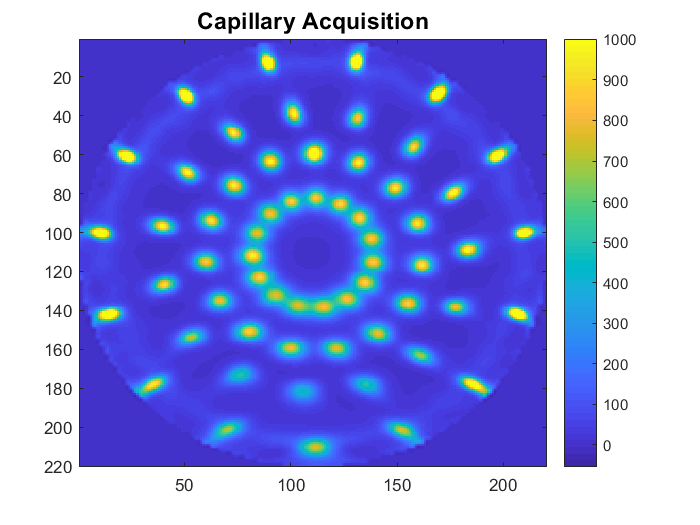
\includegraphics[width=3in]{figures/Capillary_newLRF.PNG}

\caption{The reconstructed capillary phantoms after corrections. The capillaries had 1mm diameter; each were filled with 10 MBq of $^{99m}Tc$ and were scanned for 5 minutes.}
\label{fig_ImageRes}
%\vspace{-0.2cm}
\end{figure}

\begin{figure}[!t]
%\vspace{-0.2cm}
\centering
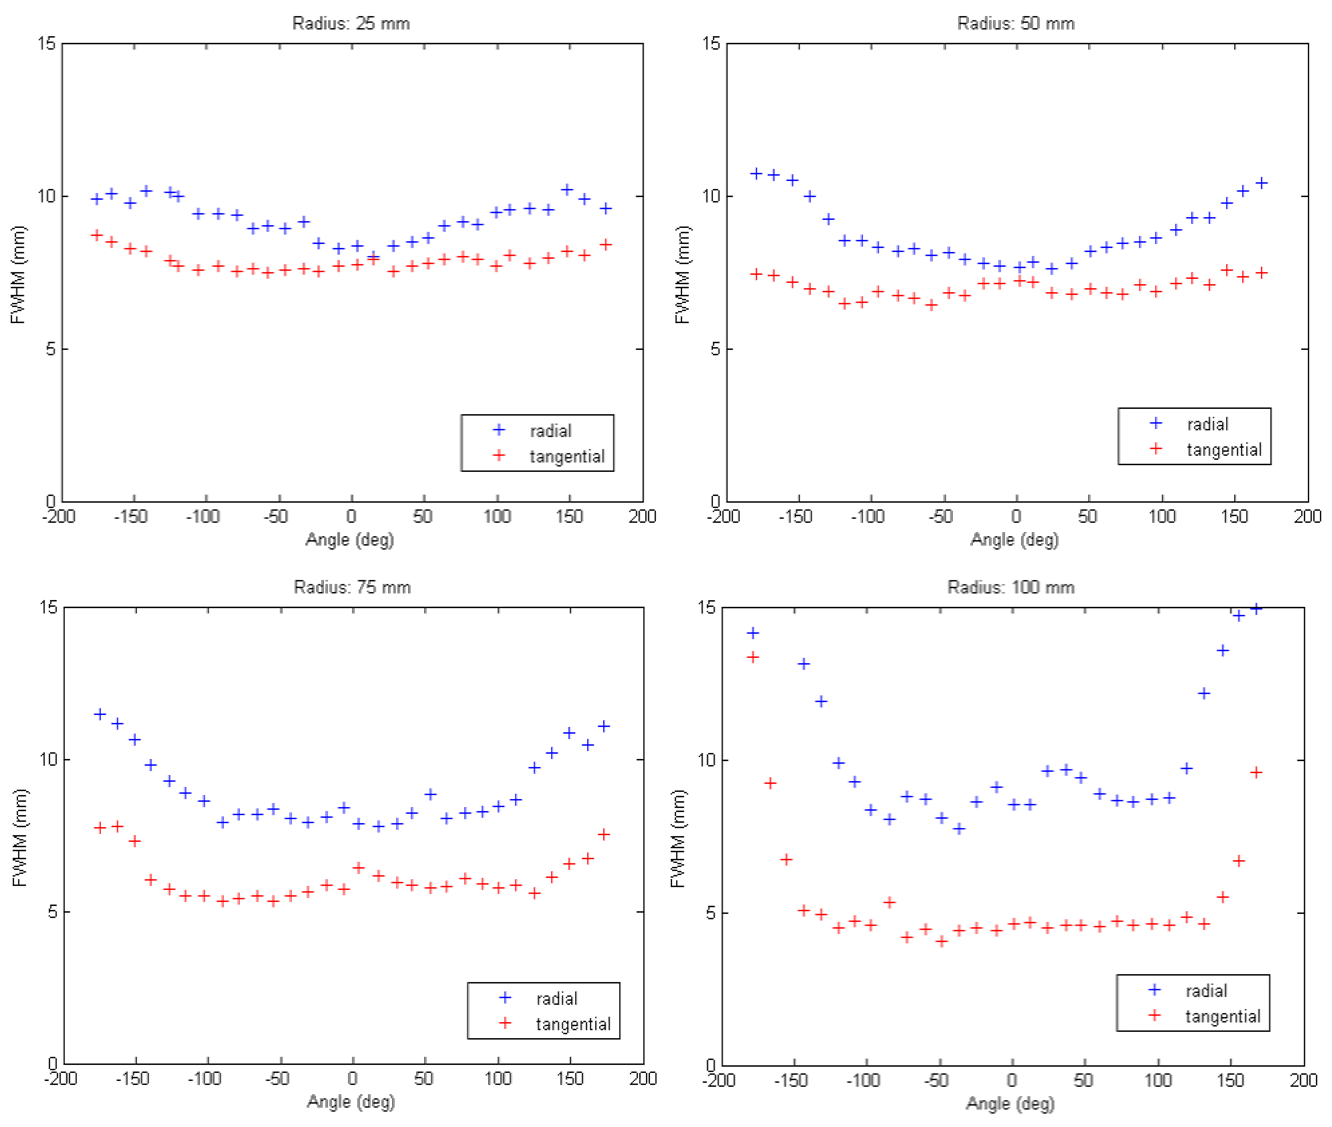
\includegraphics[width=3.4in]{figures/resolutions.png}

\caption{Resolution of capillaries at 4 radial positions against the angular position in the FOV.}
\label{fig_resolution}
%\vspace{-0.2cm}
\end{figure}

\begin{figure}[!t]
%\vspace{-0.2cm}
\centering
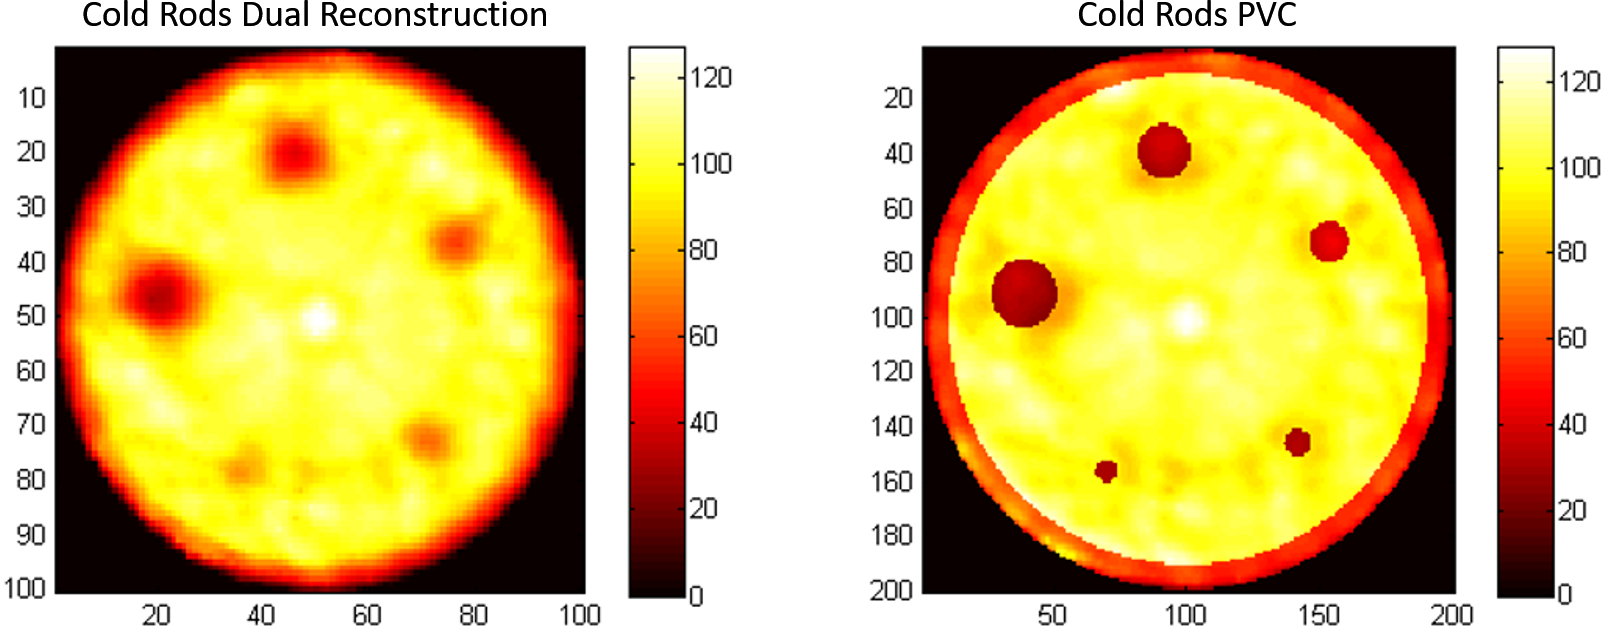
\includegraphics[width=3.5in]{figures/ColdRods.png}

\caption{Cylinder phantom of 50 MBq of activity and cold rods of diameters; 8, 10, 15, 20 and 25 mm.}
\label{fig_cold}
%\vspace{-0.2cm}
\end{figure}

\begin{figure}[!t]
%\vspace{-0.2cm}
\centering
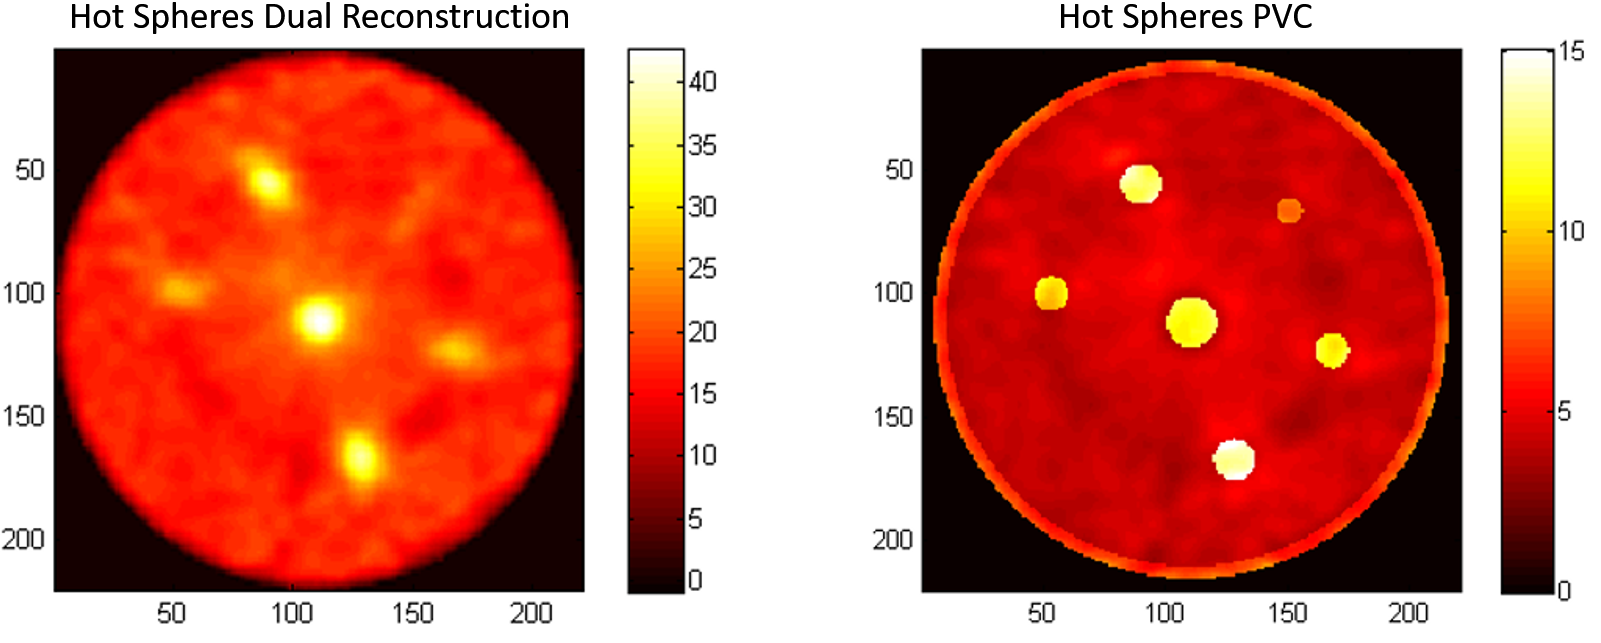
\includegraphics[width=3.5in]{figures/HotSpheres.png}

\caption{60 MBq to a ratio of 8:1 in the hot spheres of diameters; 11, 14, 17, 21 mm.}
\label{fig_Hot}
%\vspace{-0.2cm}
\end{figure}

\begin{figure}[!t]
%\vspace{-0.2cm}
\centering
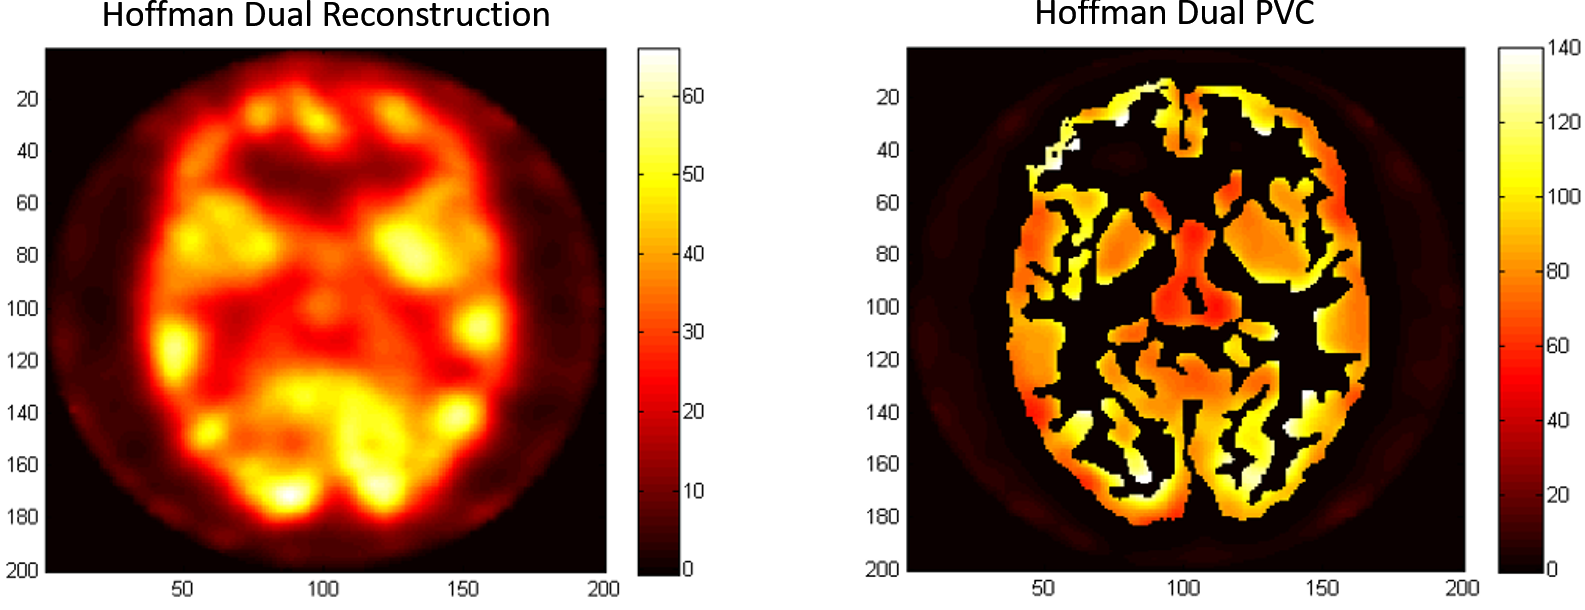
\includegraphics[width=3.5in]{figures/Hoffman.png}

\caption{2D Hoffman phantom with activity 25 MBq.}
\label{fig_Hoffman}
%\vspace{-0.2cm}
\end{figure}


\section{Conclusion and Discussion}
Overall the acquisition and reconstruction methods have demonstrated effective means of generating reconstructed images from incomplete data acquisition. We are able to correct for inhomogeneity in the detectors and produce correct projection data. The sensitivity model is able to improve image reconstruction by accounting for geometric variations across the projections. The results of this research improved the processing of INSERT projection data and introduced dual reconstruction, which can be used to benefit the system's clinical performance.
The images acquired show some limitation in the system, however we are able to produce good quality images from the SPECT system alone. Implementing the dual reconstruction has shown to improve the images, however we treat this as an extension to our system, the system is able to function and produce good quality images without this step. The INSERT detector technology has undergone preliminary characterisation of the SPECT system, \cite{8891783}, however complete MR compatibility has only been validated in the preclinical system, \cite{8612977}. Future work will set out to test the system in a clinical MR environment and to streamline calibration and acquisition procedures for routine use. The use of MR data will improve the images further and demonstrate the potential of the fully operational system.   

